% Tämä on fysiikan laboratoriotöiden selostuspohjapohja.
% Pohja ei kuitenkaan ole mikään virallinen ja oikea totuus, 
% eli muistakin pohjia voi käyttää. Tämän tarkoitus on ainoastaan 
% auttaa opiskelijoita LaTeXin alkuun.
%
% Pohjaa saa levittää ja muuttaa vapaasti. Pohjan muuttajan toivotaan 
% kuitenkin lisäävän tiedot muutoksesta ja sen ajankohdasta tämän 
% kommenttiosuuden loppuun.  
%
% Pikainen käyttöohje:
% Päivita kansilehden tiedot
% Kirjoita selostuksesi
% ATK-keskuksessa käännät koodin seuraavilla komennoilla:
% use latex
% latex selkkari.tex
% 
% Esikatsele:
% xdvi selkkari
%
% Possuksi (tiedostonimeksi selostus.ps):
% dvips -o selostus.ps selkkari
%
% Toivottavasti tämä pohja auttaa alkuun
%
% Jukka Katainen, 6.2.2004
%
\documentclass[a4paper,11pt]{article}

\frenchspacing
\usepackage[finnish]{babel}
\usepackage[utf8]{inputenc}
\usepackage{graphicx}
\usepackage[T1]{fontenc}

\begin{document}

%Tästä alkaa selkkarin kansilehti. Vaihda tilalle tarvittavat tiedot.
\begin{titlepage}
\pagestyle{empty}
\begin{center}

\vspace*{3cm}
\noindent\LARGE{\textbf{Työ 
%
%*******************************************************
%Työn numero:
55
%*******************************************************
%
\\
%
%*******************************************************
%Työn nimi:
Radioaktiivisuus ja säteily
%*******************************************************
%
}}\\
\vspace*{2cm}
Työvuoro \LARGE{\textbf{
%
%*******************************************************
%Työvuoro:
51
%*******************************************************
%
}} pari \LARGE{\textbf{
%
%*******************************************************
%Parin numero:
4
%*******************************************************
}}\\
\vspace*{1cm}
\large{
\begin{tabular}{l l}
%
%*******************************************************
%Parin opiskelijat ja opiskelijanumerot:
Juho Salmii & 80391C\\
Jukka Kemppainen & \\
%*******************************************************
%
\end{tabular}

\vspace*{1cm}
Selostuksen laati \emph{
%
%*******************************************************
% Selostuksen tekijä:
Juho Salmi
%*******************************************************
%
} \\
\vspace*{1cm}
\begin{tabular}{l l}
Mittaukset suoritettu & \textbf{
%
%*******************************************************
% Mittaukset suoritettu
11.11.2013
%*******************************************************
%
}\\
Selostus palautettu & \textbf{
%
%*******************************************************
% Selostus palautettu
18.11.2013
%*******************************************************
%
}\\
\end{tabular}
}
\end{center}
\end{titlepage}
%kansilehti loppuu tähän

%Varsinainan selkkari alkaa
\section{Johdanto}

Atomit koostuvat sen ytimeen pakkautuneista protoneista ja neutroneista sekä ulkokehällä sijaitsevistä elektroneista. Ytimen hiukkasten välillä on vahva vuorovaikutus, joka pitää atomiydintä koossa. Sähkömagneettinen vuorovaikutus saa puolestaan positiivisesti varautuneet ytimen protonit hylkimään toisiaan. Näiden voimien yhteisvaikutuksesta vain tietyn protoni- ja neutronimäärän sisältävät atomiytimet ovat stabiileja. \cite{ohje, wiki:radioaktiivisuus}

Epästabiilit atomiytimet pyrkivät stabiileiksi spontaanisti hajoamalla. Tätä kutsutaan radioaktiivisesksi hajoamiseksi. Hajoamisessa vapautuneiden hiukkasten sinkoutumista ympäristöön kutsutaan radioaktiiviseksi säteilyksi. \cite{ohje, wiki:radioaktiivisuus}

Tässä työssä tutkitaan alfa-, beeta- ja gammahajoamisia sekä -säteilyä. Alfahajoamisessa ydin emittoi kahden protonin ja neutronin muodostaman alfahiukkasen eli heliumytimen. Beetahajoamisessa protoni muuttuu neutroniksi tai päin vastoin. $\beta^-$-hajoamisessa ytimen neutroni muuttuu protoniksi vapauttaen elektronin ja antineutriinon. $\beta+$-hajoamisessa protoni muuttuu neutroniksi vapauttaen positronin ja neutriinon. Vapautuvia elektroneita tai positroneita kutsutaan beetahiukkasiksi ja -säteilyksi. \cite{ohje, wiki:radioaktiivisuus}

Alfa- ja beetahajoamisissa atomiydin voi jäädä virittyneeseen tilaan. Viritystilan lauetessa ydin emittoi viritysenergiansa gammafotonina. Tätä kutsutaan gammahajoamiseksi ja -säteilyksi. \cite{ohje, wiki:radioaktiivisuus}

Alfa- ja beetasäteilyä kutsutaan hiukkassäteilyksi, sillä niissä vapautuu hiukkasia, joilla on massa. Gammasätely on puolestaan sähkömagneettista säteilyä. \cite{ohje, wiki:radioaktiivisuus}

Eri radioaktiivisen säteilyn tyypeillä on erilaiset ominaisuudet \cite{ohje, wiki:radioaktiivisuus}. Tässä työssä tutustutaan alfa-, beeta- ja gammasäteilyn kantamaan ilmassa sekä läpäisykykyyn ja absorptioon erilaisissa väliaineissa. 

\section{Laitteisto ja menetelmät}

Säteilynilmaisin eli detektori on laite, joka tuottaa jännitepulssin havaitessaan säteilyhiukkasen. Pulssitaajuus ($\dot{n}$) on pulssimäärä ($n$) aikayksikköä kohden. Detektori ei havaitse kaikkia siihen osuvia hiukkasia. Havaitsemistodennäköisyyttä kutsutaan detektorin efektiivisyydeksi ($\epsilon$). Radioaktiivisten hajoamisten lukumäärä noudattaa Poisson-jakaumaa, joten pulssimäärän virhearviona voidaan käyttää sen neliöjuurta: $\Delta n = \sqrt{n}$.

Lähteen aktiivisuus $A$ tarkoittaa siinä tapahtuvien radioaktiivisten hajoamisten määrää aikayksikköä kohden. Aktiivisuuden yksikkö on 1/s, jonka erityisnimi on Becquerel (Bq). Aktiivisuus voidaan määrittää mittaamalla lähteen säteilyn pulssitaajuutta ($\dot{n}$). Oletetaan lähteen koko etäisyyteen nähden niin pieneksi, että lähdettä voidaan käsitellä pistemäisenä. Oletetaan lisäksi detektori niin pieneksi, että sitä voidaan kuvata tasona. Gammasäteilyn kohdalla vuorovaikutustodennäköisyys ilman kanssa on niin pieni, ettei säteilyä absorboidu merkittävästi ennen sen osumista detektoriin. Tällöin detektorin havaitsema pulssitaajuus on 

\begin{equation}
  \dot{n} = \epsilon \cdot A \cdot n_A \cdot \frac{\Omega}{4 \pi} ,
\end{equation}

jossa $n_A$ on yhdessä hajoamisessa emittoituvien gammakvanttien määrä, jossa lähde näkee detektorin. Detektorin pinta-ala on $a_d$, joten kaava voidaan kirjoittaa muotoon

\begin{equation}
  \dot{n} = \epsilon \cdot A \cdot n_A \cdot \frac{a_d}{4 \pi r^2} ,
\end{equation}

jossa $r$ on detektorin etäisyys lähteestä. Pulssitaajuus on siis kääntäen verrannollinen etäisyyden neliöön. 

Säteilyn absorptiotodennäköisyys väliaineessa kasvaa väliaineen järjestysluvun funktiona ja pienenee fotonin energian funktiona. Gammasäteilyn intensiteett $\varphi$ vaimenee säteilyn väliaineessa kulkeman matkan $x$ funktiona eksponentiaalisesti:

\begin{equation}
  \varphi(x) = \varphi_0 \cdot e^{-\mu \cdot x} ,
\end{equation}

jossa $\varphi_0$ on intensiteetti ennen väliaineeseen osumista. Matkavaimennuskerroin $\mu$ on väliaineesta ja fotonin energiasta riippuva absorptiotodennäköisyys pituusyksikköä kohden. Detektorin mittaama pulssitaajuus on suoraan verrannollinen säteilyn intensiteettiin: 

\begin{equation}
  \label{ndot}
  \dot{n} = \epsilon \cdot \varphi \cdot a_d 
\end{equation}

Osuessaan väliaineeseen, säteily ionisoi sen atomeita ja molekyylejä. Absorboitunut annos $D$ määritellään kohteeseen absorboituneen säteilyenergian ja kohteen massan suhteena: 

\begin{equation}
  D = \frac{E}{m}
\end{equation}

Absorboituneen annoksen yksikkö on J/kg, jonka erityisnimitys on Gray (Gy). Annosnopeus on absorboitunut annos aikayksikköä kohti: 

\begin{equation}
  \dot{D} = \frac{dD}{dt} = \frac {dE}{dt} \frac{1}{m}
\end{equation}

Energiaa siirtyy väliaineeseen saman verran kuin säteilyn intensiteetti vaimenee, joten annosnopeus voidaan kirjoittaa muotoon: 

\begin{equation}
  \label{annos3}
  \dot{D} = \frac{\varphi \cdot a \cdot p_{abs} \cdot \bar{E}}{m} ,
\end{equation}

jossa $a$ on tarkasteltavan tilavuusalkion pinta-ala, $p_{abs}$ fotonien absorboitumistodennäköisyys ja $\bar{E}$ fotonien keskimääräinen energia. Tarkasteltaessa pientä tilavuusalkiota voidaan absorptiotodennköisyys korjoittaa muotoon

\begin{equation}
  p_{abs} = \mu_{en} \cdot l ,
\end{equation}

jossa $\mu_{en}$ on energian absorptiotodennäköisyys pituusyksikköä kohden ja $l$ tilavuusalkion pituus. Massa voidaan puolestaan kirjoittaa puolestaan tiheyden, pinta-alan ja pituuden tulona ($\rho \cdot a \cdot l$) ja $\phi$ voidaan ratkaista kaavasta \ref{ndot}. Saadaan siis 

\begin{equation}
  \dot{D} = \frac{\dot{n} \cdot a \cdot \mu_{en} \cdot l \cdot \bar{E}}{\epsilon \cdot a_d \cdot \rho \cdot a \cdot l} = \frac{\dot{n} \cdot \bar{E}}{\epsilon \cdot a_d} \frac{ \mu_{en}}{\rho}
\end{equation}

jossa tekijää $\mu_{en}/\rho$ kutsutaan energia-absorption massakertoimeksi. Vaihtoehtoisesti voidaan pienillä etäisyyksillä mitatessa arvioida, että annosnopeus voidaan määrittää vaimentumattoman ($\dot{n}_0$) ja väliaineessa vaimentuneen ($\dot{n}_1$) pulssitaajuuden avulla. 

\begin{equation}
  \varphi \cdot a \cdot p_{abs} = \frac{\dot{n}_0-\dot{n}_1}{\epsilon}
\end{equation}

Sijoittamalla tämä kaavaan \ref{annos3} saadaan annosnopeudeksi

\begin{equation}
  \dot{D} = \frac{(\dot{n}_0-\dot{n}_1) \cdot \bar{E}}{\epsilon \cdot m} .
\end{equation}

Eri säteilyn lajien samansuuruisilla absorboituneilla annoksilla on erilaiset biologiset vaikutukset. Ekvivalenttiannos painottaa säteilyannosta eri painokertoimella kutakin säteilylajia kohden ja efektiivinen annos painottaa ekvivalenttiannosta kunkin kohde-elimen painokertoimella. Ekvivalenttiannoksen yksikkö on J/kg eli Sievert (Sv).

\cite{ohje}

\subsection{Alfa- ja beetasäteilyn mittaus}
\label{laitteisto:alfabeeta}

Alfa- ja beetasäteilyn mittauksessa säteilylähteet ja detektori on asennettu muovikoteloon, jossa säteilylähteiden etäisyyttä detektorista voidaan säätää ruuvilla ja säteilylähde voidaan vaihtaa tappia vetämällä tai työntämällä. Detektoriin kytketystä mittalaitteesta voidaan lisäksi valita mitattavaksi haluttu säteilylaji. Alfasäteilyn lähde koostuu Am-241-isotoopista ja beetasäteilyn ($\beta^-$) lähde Sr-90-isotoopista. Lähteet ovat tasomaisia, halkaisijaltaan 10 mm. Alfahiukkasten energia on noin 5,5 MeV. Beetahiukkasten maksimienergia 546 keV ja keskimääräinen energia 196 keV. \cite{ohje}


\subsection{Gammasäteilyn mittaus}
\label{laitteisto:gamma}

Gammasäteilyn mittauksessa käytetään säteilylähteenä Co-60-isotooppia, joka $\beta^-$-hajoamisella muuttuu Ni-60-isotoopiksi. Hajoamisen jälkeen ydin jää viritystilaan, jonka purkautuessa emittoituu kaksi gammakvanttia energioiltaan 1173 keV ja 1332 keV. Detektorina käytetään tuikeilmaisinta, jonka pohjan pinta-ala on $5,07 cm^2$. Detektori havaitsee noin 36 \% tuikekiteeseen osuvista gammakvanteista. Annosnopeuden mittaukseen käytetään Geiger-Muller-putkeen perustuvaa dosimetria. \cite{ohje}



\section{Tulokset}

\subsection{Alfa- ja beetasäteily}
\label{tulokset:alfabeeta}

Mitataan alfalähteen säteilyn pulssitaajuus 5 mm etäisyydeltä vaimentamattomana sekä mylarkalvon kanssa. 
\begin{table}[ht]
\begin{center}
\caption{Alfalähteen aiheuttama pulssitaajuus 5mm etäisyydeltä}
\begin{tabular}{ | r | l | }
  \hline 
  vaimentumaton & $4000 \pm 200 Bq$ \\ \hline
  mylarkalvon kanssa & $0,25 \pm 0,25 Bq$ \\ \hline
\end{tabular}
\end{center}
\end{table}

Mitataan alfasäteilyn kantama ilmassa siirtämällä alfalähdettä kauemmas detektorista. Saadaan, että $23 \pm 1 mm$ etäisyydellä detektori ei havaitse kuin satunnaisia hajoamisia, joten etäisyys voidaan katsoa alfasäteilyn kantamaksi. 

Mitataan beetalähteen säteilyn pulssitaajuus 5mm etäisyydeltä vaimentamattomana, mylarkalvon ja pleksilevyn kanssa.
\begin{table}[ht]
\begin{center}
\caption{Beetalähteen aiheuttama pulssitaajuus 5mm etäisyydeltä}
\begin{tabular}{ | r | l | }
  \hline
  vaimentumaton & $350 \pm 50 Bq$ \\ \hline
  mylarkalvon kanssa & $350 \pm 50 Bq$ \\ \hline
  pleksilevyn kanssa & $125 \pm 25 Bq$ \\ \hline
\end{tabular}
\end{center}
\end{table}
   
Mitataan beetasäteilyn vaimenemista siirtämällä beetalähde niin kauas detektorista kuin mittalaitteella on mahdollista. Saadaan maksimietäisyydellä $83 \pm 0,5 mm$ pulssitaajuudeksi $75 \pm 25 Bq$. 

\subsection{Gammasäteily}
\label{tulokset:gamma}

Mitataan gammalähteen pulssien lukumäärää eri etäisyyksiltä tasavälisesti $1/r^2$ suhteen kymmenen sekunnin ajan. 

\begin{table}[ht]
\begin{center}
\caption{Gammalähteestä mitattujen pulssien määrä eri etäisyyksiltä 10 s aikana}
\begin{tabular}{ | r | l | }
  \hline
Etäisyys (cm) & Havaitut pulssit (kpl) \\ \hline
5.0 & 2704 \\ \hline
5.3 & 2474 \\ \hline
5.7 & 2061 \\ \hline
6.1 & 1830 \\ \hline
6.7 & 1552 \\ \hline
7.4 & 1320 \\ \hline
8.5 & 1005 \\ \hline
10.3 & 743 \\ \hline
14.1 & 523 \\ \hline
40.0 & 319 \\ \hline
\end{tabular}
\end{center}
\end{table}

Etäisyyden virheeksi arvioidaan $\pm 0,2 cm$.

\begin{figure}[ht]
\centering 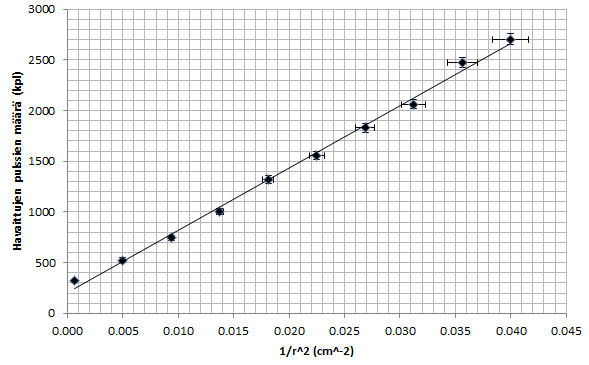
\includegraphics[width=0.8\textwidth]{gamma1}
\caption{Tapahtumasuuntautunut maailmankuva. \label{gamma1}}
\end{figure}

\clearpage

Mitataan gammalähteen pulssien lukumäärä 20 cm etäisyydeltä 100 s ajan eri määrällä lyijylevyistä valmistettuja absorptiolevyjä. 

\begin{table}[ht]
\begin{center}
\caption{Gammalähteestä mitattujen pulssien määrä 20 cm etäisyydeltä 100 s aikana eri lyijykerroksen paksuuksilla}
\begin{tabular}{ | r | l | }
  \hline
Lyijyn määrä (cm) & Havaitut pulssit (kpl) \\ \hline
0 & 4000 \\ \hline
2 & 3797 \\ \hline
4 & 3801 \\ \hline
6 & 3554 \\ \hline
8 & 3535 \\ \hline
12 & 3330 \\ \hline
16 & 3315 \\ \hline
20 & 3003 \\ \hline
28 & 2809 \\ \hline
36 & 2655 \\ \hline
50 & 2576 \\ \hline
80 & 2193 \\ \hline

\end{tabular}
\end{center}
\end{table}

Mitataan dosimetrillä säteilyannosta työskentelypaikalta lyijytiilien kanssa, ilman lyijytiiliä sekä 5 cm päässä gammalähteestä. 

\begin{table}[ht]
\begin{center}
\caption{Beetalähteen aiheuttama pulssitaajuus 5mm etäisyydeltä}
\begin{tabular}{ | r | l | }
  \hline
  lyijytiilien kanssa & $0,18 \pm 0,01 Sv$ \\ \hline
  ilman lyijytiiliä & $0,18 \pm 0,01 Sv$ \\ \hline
  5 cm päässä lähteestä & $0,50 \pm 0,05 Sv$ \\ \hline
\end{tabular}
\end{center}
\end{table}

\clearpage

\section{Yhteenveto ja pohdinnat}

Havaitaan, että alfasäteily pysähtyy ohueenkin väliaineeseen, siinä missä beetasäteily läpäisee vähän paksummankin väliaineen. Gammasäteily puolestaa läpäisee jopa paksumman lyijykerroksen. Samalla tavalla käyttäytyvät myös säteilytyyppien kantamat. Nämä on pidettävä mielessä säteilyltä suojautuessa. 

Mittauksia tehdessä, olivat tutkimuksen tekijät pääsääntöisesti suojattu säteilyltä, eikä lähelläkään säteilylähdettä ollut vaarallisia annosnopeuksia. Ainoa elin, joka joutui lähelle säteilylähdettä oli käsi, ja sen efektiiviset painokertoimet ovat pieniä. 


%Kirjallisuuviitteet
\begin{thebibliography}{99}
% Kirjallisuus viitteet tähän tapaan:
%\item{R.W. Robinnet, Quantum Mechanics, Oxford University Press, 1997}

\bibitem{ohje} Harjoitustyöohje: Työ 55 Radioaktiivisuus ja säteily, http://physics.aalto.fi/pub/kurssit/Tfy-3.15xx/materiaali/55.pdf [Viitattu 18.11.2013]
\bibitem{wiki:radioaktiivisuus} Wikipedia-artikkeli radioaktiivisuudesta, http://fi.wikipedia.org/wiki/Radioaktiivisuus [Viitattu 18.11.2013]

\end{thebibliography}

%liitteet numeroituna
\section*{Liitteet}
\begin{enumerate}
%Liitteet tähän tapaan
\item{Mittauspöytäkirja}\label{mittaus}

\end{enumerate}

\end{document}
